\section{Methods}

\begin{figure}[h]
    \centering
    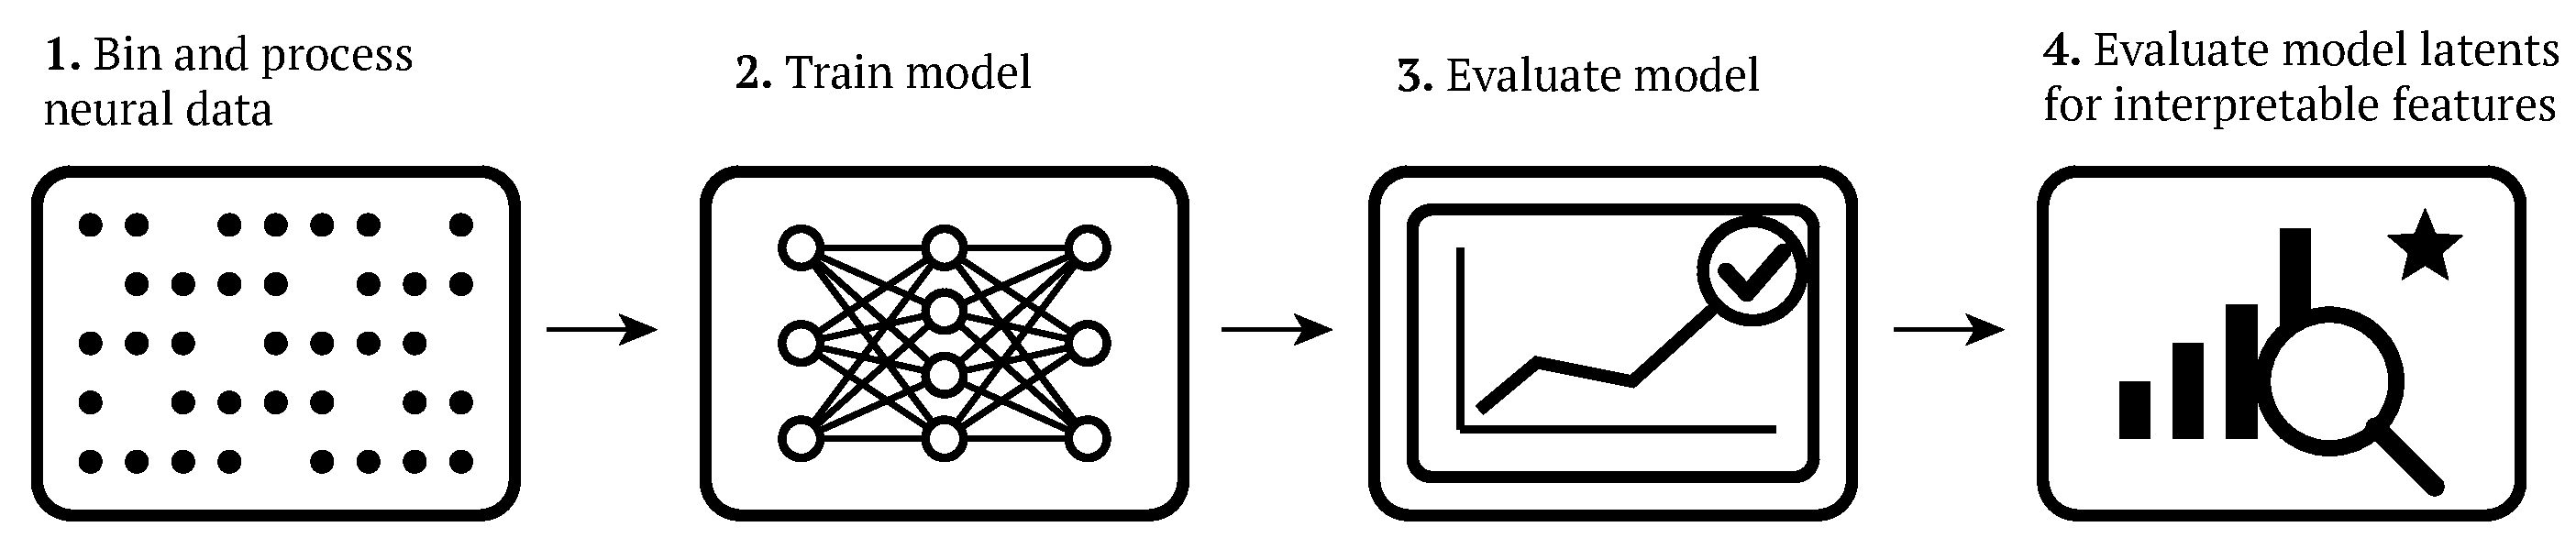
\includegraphics[width=\linewidth]{figures/mini_pipeline.pdf}
    \caption{
        \textbf{The MINI pipeline.} \\
        \small The MINI pipeline contains 4 steps: 1) Spatiotemporal binning and processing of neural data; 2) Training a MINI model; 3) Evaluating, and optionally re-training, the model; 4) Evaluating the model latents for interpretable features. Depending on a user's preference, steps 1-3 (including model re-training), can be either semi- or fully-automated.
    }
    \label{fig:mini_pipeline}
\end{figure}

\subsection{Pipeline Overview}

- Overall: MINI takes in high-dimensional neural data and outputs latents to evaluate

- For a user, the full, semi-automated pipeline is as follows:
\begin{enumerate}
    \item Data preprocessing
    \begin{itemize}
        \item Spatiotemporally bin and normalize
        \begin{itemize}
            \item MINI has a convenience function to do this directly from output of common spikesorters (kilosort), where we bin unit spikes given a specified timebin and optionally normalize (z-score or max) dataset across time and/or unit
            \begin{itemize}
                \item (and similar approach could be applied to output from common calcium imaging processing (e.g. Suite2p))
            \end{itemize}
        \end{itemize}
    \end{itemize}
    
    \item Model training
    \begin{itemize}
        \item Hyperparameter optimization
        \item By default no validation set, but can be added if we want to e.g. apply to other recordings of same animal, though this is not generally recommended (just train a freshie)
    \end{itemize}
    
    \item Model evaluation
    \begin{itemize}
        \item (We implement all metrics from SAEBench which are not language-model specific, plus a couple of our own)
        \item L0 of latents
        \item R\textsuperscript{2} (var explained) and cos sim of reconstruction-to-actual neural activity for each spatial bin, and each temporal bin
        \item Latent density histogram (as in SAEBench)
        \item Variance explained of overall reconstruction from each latent (variance shouldn't be in just a few features) ?
        \item Spectral frequency analysis to ensure temporal frequency content is preserved?
    \end{itemize}
    
    \item Feature evaluation
    \begin{itemize}
        \item When a latent is deemed sufficiently interpretable, we call this a feature.
        \item Interactive plots showing feature activation patterns across time and experimental conditions.
        \item We evaluate its decoding performance?
        \item Export functionality.
    \end{itemize}
\end{enumerate}


\subsection{Model architecture}

\begin{figure}[h]
    \begin{minipage}{0.68\linewidth}
    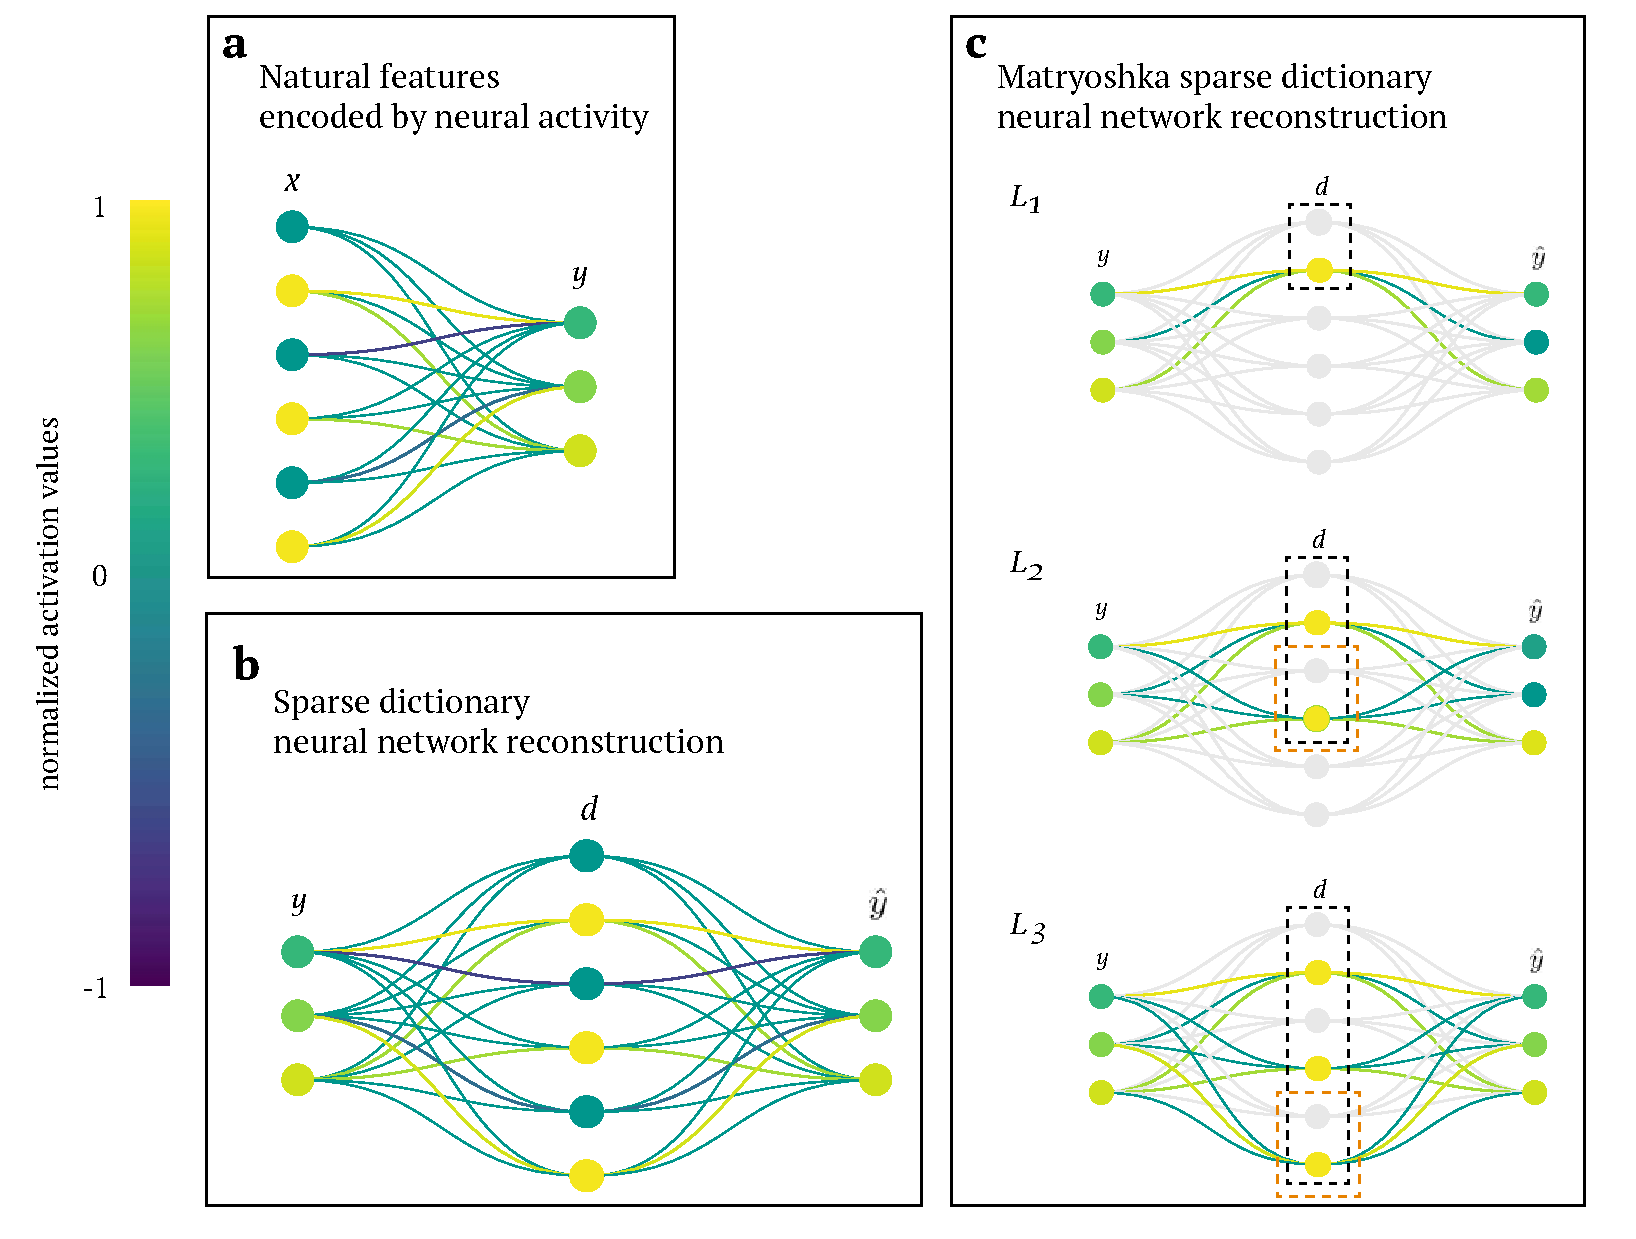
\includegraphics[width=\linewidth]{figures/sdnn_arch.pdf}
    \end{minipage}%
    \begin{minipage}{0.33\linewidth}
    \caption{
        \textbf{MINI's sparse dictionary neural network architecture.} \\
        \small (\textbf{a}) Natural features $x$ get encoded by neural activity $y$. (\textbf{b}) A sparse dictionary neural network attempts to recreate neural activity $\hat{y}$ from $y$. If $\hat{y}$ tries to recreate $y$ exactly, then the model is an autoencoder, while in other situations it may be a transcoder or crosscoder. ()\textbf{c}) A Matryoshka spare dictionary neural network segments the latent space into multiple levels, each of which attempts to do a full reconstruction of the target neural activity. In this case, latents exclusive to the highest-level will often correspond to high-level features (e.g. a round object), while latents exclusive to the lowest-level will often correspond to low-level features (e.g. a basketball).
    }
    \label{fig:sdnn_arch}
    \end{minipage}
\end{figure}

\begin{itemize}
    \item Usefulness of SDL methods in Mech interp.
    
    \item Variant of MSAE as variant of SAE.
    \begin{itemize}
        \item Briefly mention other archs tried: batchTopK winner for sparsity enforcement.
    \end{itemize}
    
    \item In addition to MSAE levels width, briefly mention hyperparameters, expound in Appendix.
    \begin{itemize}
        \item topk per level, loss X per level, seq len for neural data, seq len for latent space used with transformer layer in decoder
    \end{itemize}
    
    \item Show latex formulas for encoder, decoder, total loss.
\end{itemize}
